\chapter{Supplementary material for \autoref{chap:rys}}
\section{Supplementary figures}

\begin{sidewaysfigure}[!h]
    \makebox[\textwidth][c]{\includegraphics[width=1.2\textwidth]{rys/synteny2.png}}    
    \caption{{\bf Synteny Database output for the syntenic region containing \textit{D. rerio} npat}}
    Dre\#: \textit{Danio rerio chromosome \#}
    Hsa\#: \textit{Homo sapiens chromosome \#}

    The relative position of the displayed genomic neighbourhoods on their chromosome scaffolds is displayed inset, top right. \textit{D. rerio} npat is highlighted with a red square, visible on the right of the selected Dre15 region, annotated ``im:6901964''. \textit{H. sapiens} NPAT is highlighted similarly on the left of Hsa11. landmarks of the duplication and rearrangement event that brackets the position of npat on Dre15 are highlighted with red lines.

    On the scaffold of \textit{H. sapiens} chromosome 11, NPAT occurs upstream of the highlighted duplication cluster bracketed by ARCN1 and MIZF. Zebrafish npat is located in the midst of this rearranged, duplicated cluster, but does not appear to have been duplicated itself; at least if it was, no paralogue can be found by syntenic or similarity analysis.
    \label{synteny}
\end{sidewaysfigure}


\begin{figure}[!h]
    \makebox[\textwidth][c]{\includegraphics[width=1.\textwidth]{rys/npat transcripts.jpg}}    
    \caption{{\bf npat is overexpressed in \textit{rys}}} 
    \label{npatrtpcr}
\end{figure}

\begin{figure}[!h]
    \makebox[\textwidth][c]{\includegraphics[width=1.\textwidth]{rys/cmzfailure.png}}    
    \caption{{\bf 10dpf mutant \textit{rys} RPCs are mitotic}} MIP 14\si{\micro\metre} coronal cryosections through representative sib (left panels) and \textit{rys} eyes at 10dpf, 7 days after an 8hr BrdU pulse at 3dpf. Note that few labelled \textit{rys} cells have entered the specified retinal layers.
    \label{rysmitosis}
\end{figure}

\begin{figure}[!h]
    \makebox[\textwidth][c]{\includegraphics[width=1.\textwidth]{rys/rys_4c4.png}}    
    \caption{{\bf 4C4-positive microglia engulf \textit{rys} mutant RPCs}} 
    \label{phagocytosis}
\end{figure}


\begin{figure}[!h]
    \makebox[\textwidth][c]{\includegraphics[width=1.\textwidth]{rys/morpholinoqPCR.png}}    
    \caption{{\bf Morpholinos directed to npat result in histone transcript overexpression similar to \textit{rys}}} 
    \label{morpholinoRTPCR}
\end{figure}


\begin{figure}[!h]
    \makebox[\textwidth][c]{\includegraphics[width=.9\textwidth]{rys/chr_unique_positions.png}}    
    \caption{{\bf Novel nucleosome positions in \textit{rys} occur in similar numbers to those lost from sibs.}}
    Counts of positions found in sib but not \textit{rys} (red bars, represented as negative numbers, as these are `lost' in \textit{rys}) and those found in \textit{rys} but not sib (blue bars, `gained'). The magnitude of the difference between the counts is represented with a yellow bar.
    \label{diffposdist}
\end{figure}

\begin{figure}[!h]
    \makebox[\textwidth][c]{\includegraphics[width=.75\textwidth]{rys/bghmm.png}}    
    \caption{{\bf Test likelihoods for background HMMs trained on \textit{D. rerio} genome partitions}}
    \label{BHMMlh}
\end{figure}

\begin{figure}[!h]
    \makebox[\textwidth][c]{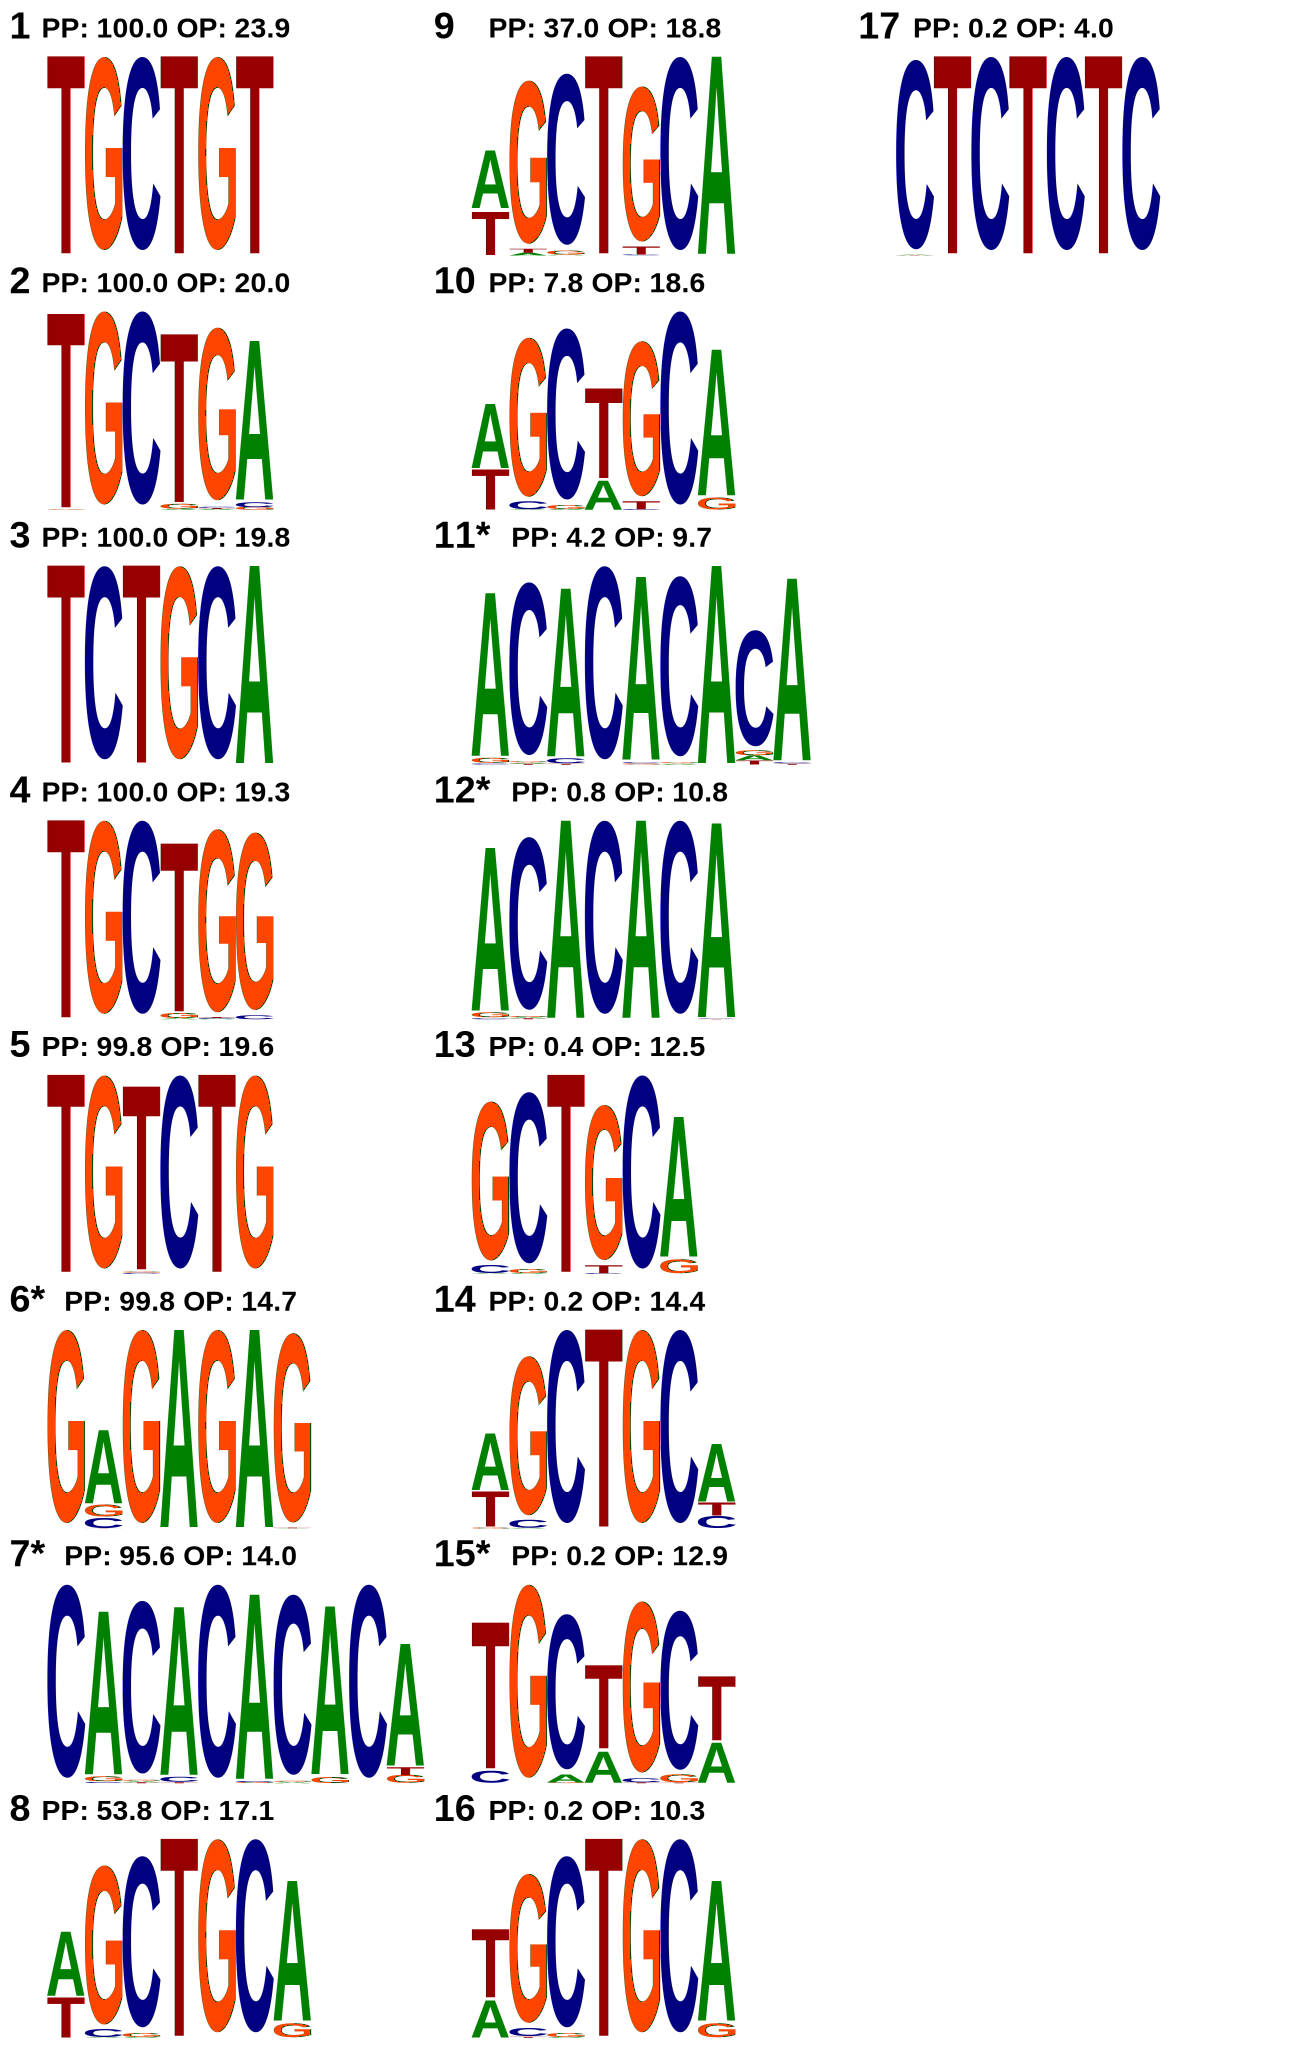
\includegraphics[width=.75\textwidth]{rys/combined_e_srcs.png}}    
    \caption{{\bf PWM sources detected in combined sib and rys differential sources.}}
    Counts of positions found in sib but not rys (red bars, represented as negative numbers, as these are `lost' in rys) and those found in rys but not sib (blue bars, `gained'). The magnitude of the difference between the counts is represented with a yellow bar.
    \label{combinedmotifs}
\end{figure}

\FloatBarrier

\section{Supplementary tables}

\begin{table}[!ht]
    \caption{Evidence for Normal vs. Log-Normal models of layer and lineage contribution}
    \begin{tabular}{|l|l|l|l|l|l|} 
        \hline
        {\bf Morpholino} & {\bf Measurement} & {\bf Separate logZ} & {\bf Combined logZ} & {\bf logZR} & {\bf $\sigma$ sign.}\\ \hline \hline
        ATG & CMZ pop. & -236.4 ± 2.3 & {\bf -198.3 ± 2.2} & -38.1 ± 3.2 & 12.1 \\ \hline
        ATG & Total sectional pop. & -412.4 ± 7.8 & {\bf -225.3 ± 4.9} & -187.1 ± 9.2 & 20.3 \\ \hline
        ATG & Sectional pop. per CMZ cell & {\bf -70.18 ± 0.86} & -78.0 ± 0.86 & 7.8 ± 1.2 & 6.4 \\ \hline
        ATG & Dorsal CMZ pop. & -169.5 ± 1.4 & {\bf -151.75 ± 0.8} & -17.8 ± 1.6 & 11.2 \\ \hline
        ATG & Ventral CMZ pop. & -223.1 ± 1.5 & {\bf -165.3 ± 1.0} & -57.8 ± 1.8 & 32.5 \\ \hline
        ATG & Nuclear volume & -290.6 ± 1.8 & {\bf -192.7 ± 1.8} & -97.9 ± 2.5 & 39.6 \\ \hline
        ATG & Nuclear sphericity & {\bf -186.13 ± 0.79} & -215.66 ± 0.57 & 29.53 ± 0.97 & 30.3 \\ \hline
        Spl & CMZ pop. & -272.6 ± 2.4 & {\bf -197.0 ± 2.6} & -75.7 ± 3.6 & 21.2 \\ \hline
        Spl & Total sectional pop. & -455.9 ± 8.3 & {\bf -205.6 ± 4.7} & -250.3 ± 9.5 & 26.3 \\ \hline
        Spl & Sectional pop. per CMZ cell & -87.04 ± 0.17 & {\bf -66.22 ± 0.29} & -20.82 ± 0.34 & 62.0 \\ \hline
        Spl & Dorsal CMZ pop. & -226.2 ± 1.7 & {\bf -171.0 ± 1.1} & -55.2 ± 2.0 & 27.7 \\ \hline
        Spl & Ventral CMZ pop. & -234.97 ± 0.81 & {\bf -222.3 ± 1.7} & -12.7 ± 1.9 & 6.8 \\ \hline
        Spl & Nuclear volume & -277.5 ± 1.6 & {\bf -223.2 ± 2.1} & -54.3 ± 2.7 & 20.4 \\ \hline
        Spl & Nuclear sphericity & -94.3 ± 1.1 & {\bf -67.71 ± 0.39} & -26.6 ± 1.1 & 23.2 \\ \hline
    \end{tabular}
   
    \begin{flushleft}logZ: logarithm of p(D), the marginal likelihood of the data, or model evidence.  Largest evidence values bolded. logZR: evidence ratio; positive values in favour of stable model.
    \end{flushleft}
    \label{morpholinoev}
\end{table}
